\documentclass[12pt, a4paper]{article}

% =========
% packages		
% =========
\usepackage[utf8]{inputenc}
\usepackage{geometry} % page size
\usepackage{fancyhdr} % page style
\usepackage{float} % force image location
\usepackage{graphicx, wrapfig, caption, subcaption} % figures
\usepackage{amsmath, mathtools, esvect} % math 
\usepackage{amssymb, amsfonts, amsthm}  % math
\usepackage{xcolor} % colour
\usepackage{empheq} % emphasize equations 
\usepackage[most]{tcolorbox} % config box
\usepackage{hyperref} % clickable files
\usepackage{listings} % environment code

% =============
% student name
% =============
\newcommand{\student}{{Jhon Charaja}}
\newcommand{\course}{{Legged robots}}
\newcommand{\labnumber}{{1}}

% ===========
% make title
% ===========
\renewcommand{\maketitle}{%
	\thispagestyle{empty}
	\begin{figure}
		\hfill
		
\includegraphics[height=.1\textheight]{images/horizontal_fotografico_com_subtitulo_ingles.pdf}
	\end{figure}
	
	\noindent
	\rule{17cm}{0.05cm}\\[0.3cm]
	\textbf{Name}: \student \hfill \textbf{Laboratory number}: \labnumber\\[0.1cm]
	\textbf{Course}: \course \hfill \textbf{Date}: \today\\
	\rule{17cm}{0.05cm}
	\vspace{0.5cm}	
}

% ==============
% page settings
% ==============
\geometry{%
  total={210mm,300mm},
  left   = 20mm,
  right  = 20mm,
  top    = 30mm,
  bottom = 30mm,
}
\pagestyle{fancy}
\fancyhf{}
\lhead{\textit{\course}}
\cfoot{-~\thepage~-}
%\lfoot{\textit{Lab}:~\labnumber}
\renewcommand{\headrulewidth}{0.5pt}
\renewcommand{\footrulewidth}{0.5pt}

\renewcommand{\thesection}{\arabic{section}}
\renewcommand{\thesubsection}{\thesection.\arabic{subsection}}
\renewcommand{\thesubsubsection}{\thesubsection.\arabic{subsubsection}}

% =========
% my colors
% =========
\definecolor{codegreen}{rgb}{0,0.6,0}
\definecolor{codegray}{rgb}{0.5,0.5,0.5}
\definecolor{codepurple}{rgb}{0.58,0,0.82}
\definecolor{backcolour}{rgb}{0.95,0.95,0.92}

% =============
% caption setup
%==============
\captionsetup{justification=centering}

% =============
% listing setup
% =============
\renewcommand{\lstlistingname}{Algorithm}% Listing -> Algorithm
\lstdefinestyle{my_style}{
    backgroundcolor=\color{backcolour},   
    commentstyle=\color{codegreen},
    keywordstyle=\color{magenta},
    numberstyle=\tiny\color{codegray},
    stringstyle=\color{codepurple},
    basicstyle=\ttfamily\footnotesize,
    breakatwhitespace=false,         
    breaklines=true,                 
    captionpos=b,                    
    keepspaces=false,                 
    numbers=none,                    
    numbersep=5pt,                  
    showspaces=false,                
    showstringspaces=false,
    showtabs=false,                  
    tabsize=1
}
\lstset{style=my_style}

% =================
% pdf configuration
% =================
\hypersetup{%
pdftitle   = {Jhon~Charaja~lab~1},
pdfauthor  = {Jhon~Charaja},
colorlinks = true,
linkcolor  = blue,
urlcolor   = blue,
citecolor  = blue,
bookmarks  = true,
}


\begin{document}
%\maketitle
\section{Decentralized control}
\subsection{Sinusoidal reference generation}
\begin{lstlisting}[language=Python,caption=Function to generate sinusoidal reference.]
def sine_reference_generator(a, f, t):
    """
    Info: generates a sine signal.

    Inputs: 
    ------
        - a: amplitude [rad]
        - f: frecuency [hz]
        - t: simulation time [sec]
    Outputs:
    -------
        - sine signal
    """
    w = 2*np.pi*f               # [rad/s]
    q = a*np.sin(w*t)           # [rad]
    dq = a*w*np.cos(w*t)        # [rad/s]
    ddq = -a*w*w*np.sin(w*t)    # [rad/s^2]

    return q, dq, ddq
\end{lstlisting}

\begin{lstlisting}[language=Python,caption=Main code.]
#!/usr/bin/env python3
# ===============================================================
#	Curso   :   Legged robots
# 	Alumno  :   Jhon Charaja
#   Lab     :   2 (Joint space motion control)
#   Activity:   1.1
# 	Info	:	Generate sinusoidal joint reference for ur5 robot
# ===============================================================

# =============
#   Libraries
# ============= 
import os
import rospy
import pandas as pd
import numpy as np
from sensor_msgs.msg import JointState
from lab_functions import *

# =========================
#   Configuration of node
# =========================
# create a node: 
rospy.init_node("node_sinusoidal_reference_generation")

# public in topic /joint_states	to send joint data	
pub = rospy.Publisher('joint_states', JointState, queue_size=1000)

# loop rate (in Hz)
rate 	= rospy.Rate(100)		# 100 [Hz]
dt 		= 1e-2					# 10  [ms]

# joints name of UR5 robot
jnames = ['shoulder_pan_joint', 'shoulder_lift_joint', 'elbow_joint','wrist_1_joint', 'wrist_2_joint', 'wrist_3_joint']

# object(message) type JointState
jstate = JointState()

# ==========================================
#   Set initial joint configuration of UR5
# ==========================================
# initial configuration: position, velocity and acceleration 
q0 =   np.array([np.pi, -np.pi/8,  -np.pi/6, 0.0, 0.0, 0.0])
qd0 =  np.array([    0.0, 0.0, 0.0, 0.0, 0.0, 0.0])
qdd0 = np.array([    0.0, 0.0, 0.0, 0.0, 0.0, 0.0]) 

# desired trajectory: position, velocity and acceleration
q_des = np.zeros(6)
dq_des = np.zeros(6)
ddq_des = np.zeros(6)

# =============
#   Save data
# =============
# directory to save data
origin 	= '../data/'
suffix 	= 'exp1.1'
pwd = os.path.dirname(os.path.realpath(__file__))
folder = os.path.join(pwd, origin, suffix)

# creates folder if it does not exist
if not os.path.exists(folder):
    os.makedirs(folder)

column_names = [
    'q1_des', 'q2_des', 'q3_des', 'q4_des', 'q5_des', 'q6_des',
    'dq1_des', 'dq2_des', 'dq3_des', 'dq4_des', 'dq5_des', 'dq6_des',
    'ddq1_des', 'ddq2_des', 'ddq3_des', 'ddq4_des', 'ddq5_des', 'ddq6_des' 
]

df = pd.DataFrame(columns=column_names)
file_name = 'data'
path = os.path.join(folder, file_name)

df.to_csv(path, index=False) 

#===============
#   Simulation
#===============
t = 0.0            # [sec] 
sim_duration = 5.0 # [sec]
sine_duration = 4.0 # [sec]

while not rospy.is_shutdown():
    # generate sine or step joint reference
    if t<=sine_duration:
        # second link
        q_des[1], dq_des[1], ddq_des[1] = sine_reference_generator(1, 0.2, t)
        # fifth link
        q_des[4], dq_des[4], ddq_des[4] = sine_reference_generator(1.5, 0.4, t)
    else:
        # second link
        q_des[1], dq_des[1], ddq_des[1] = step_reference_generator(q_des[1])
        # fifth link
        q_des[4], dq_des[4], ddq_des[4] = step_reference_generator(q_des[4])

    # publish message
    jstate.header.stamp = rospy.Time.now()
    jstate.name 		= jnames			# Joints position name
    jstate.position 	= q_des
    jstate.velocity 	= dq_des
    pub.publish(jstate)

    # update time
    t = t + dt
    
    if t>=sim_duration:
        # stop simulation
        print("stopping rviz ...")
        break

    # Append data
    row = tl(q_des) + tl(dq_des)+tl(ddq_des)
    # Fix for redimensionality
    df_row = pd.DataFrame.from_dict(dict(zip(column_names, tl(np.expand_dims(np.array(row), axis = 1)))))
    df.append(df_row, sort = False).to_csv(path, index=False, mode = 'a', header=False)     
    rate.sleep()
\end{lstlisting}


\begin{figure}
    \centering
    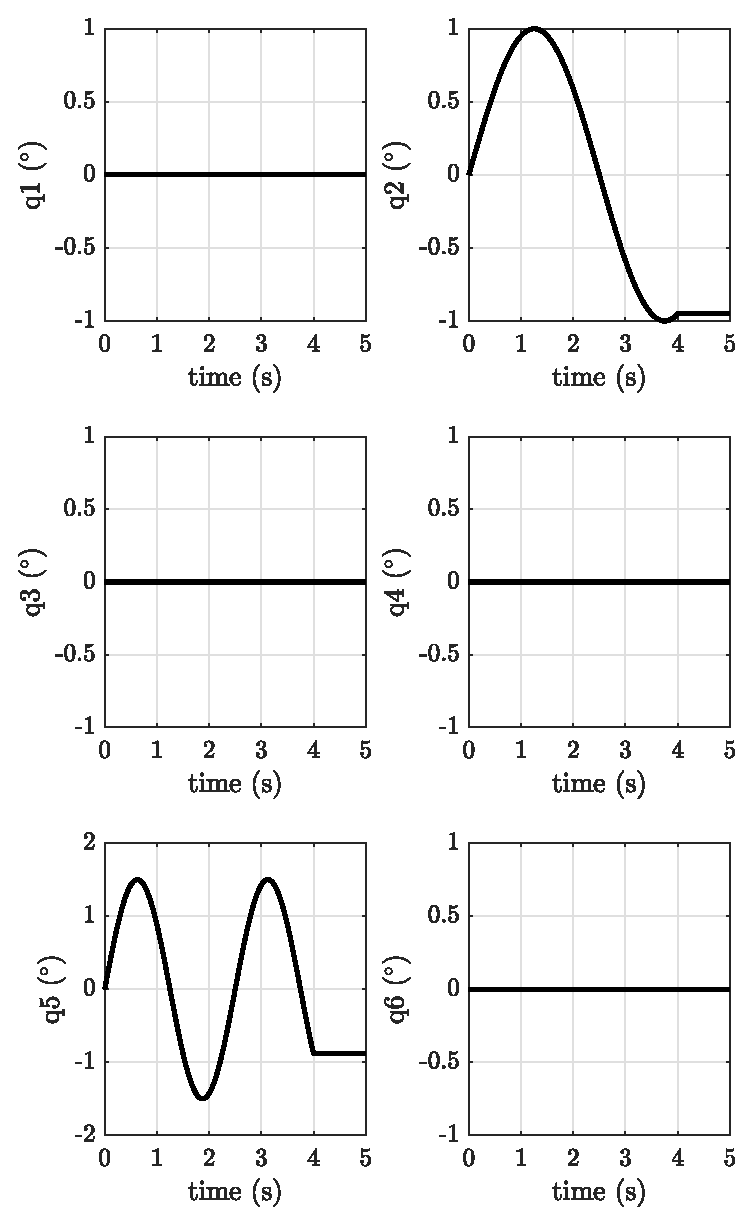
\includegraphics{images/exp1.1/joint_position.eps}
    \caption{Joint position}
    \label{fig:joint_position}
\end{figure}

\end{document}
